\subsection{Structural Robustness under Random Failure}
\label{sec:random-failure}

\subsubsection{Simulation and theoretical
reference}\label{simulation-and-theoretical-reference}

We compute all removal states by reversing each fixed removal order and
adding edges or nodes with a union-find structure, following the
reverse-addition approach of Newman--Ziff \cite{newman2000efficient}. Each returned array
is indexed by the number removed. For semantic duplicates on one
endpoint pair, connectivity changes only when the first surviving
relation is added. This implementation yields largest-component size,
component count and isolated-node count, together with surviving
structural and semantic edge counts.

We compare the curves with a generating-function prediction based on the
original empirical structural degree distribution. Define
$g_0(z)=\sum_k p_k z^k$ and $g_1(z)=g_0'(z)/g_0'(1)$. For edge retention
$q$, the reference solves $u=1-q+qg_1(u)$, taking the nontrivial solution
where it exists. Bond robustness is $1-g_0(u)$; site robustness under node
retention $q$ is $q[1-g_0(u)]$. We use the actual retained fraction after
integer rounding. These are configuration-model approximations, not exact
identities for a finite, typed biological network. Fixed-count deletion
also differs slightly from independent Bernoulli retention at finite size.

\subsubsection{Standard-graph results}\label{standard-graph-results}

The 5,000-node graph is initially connected. Under random edge removal,
most nodes remain in its largest component even after substantial
relation loss. At f=0.50, mean S is 0.98218 with sample SD 0.00128. At
f=0.90, it is 0.81540 $\pm$ 0.00366, and at f=0.99 it falls to 0.11222 $\pm$
0.01592. Thus the largest component remains large over much of the
sampled damage range but loses most original nodes at extreme edge
removal.

\begin{longtable}[]{@{}lrrrr@{}}
\caption{Random-failure robustness on the 5,000-node graph.}\label{tab:a-random}\\
\toprule\noalign{}
Removal & f & Mean S & Sample SD & GF reference \\
\midrule\noalign{}
\endhead
\bottomrule\noalign{}
\endlastfoot
Edge & 0.50 & 0.98218 & 0.00128 & 0.98213 \\
Edge & 0.90 & 0.81540 & 0.00366 & 0.81431 \\
Edge & 0.99 & 0.11222 & 0.01592 & 0.12578 \\
Node & 0.50 & 0.49252 & 0.00345 & 0.49106 \\
Node & 0.90 & 0.08474 & 0.00351 & 0.08143 \\
\end{longtable}

Figure~\ref{fig:a-random} shows the random edge and node curves with their configuration-model references.

\begin{figure}[htbp]
\centering
\begin{subfigure}[t]{0.49\linewidth}
\centering
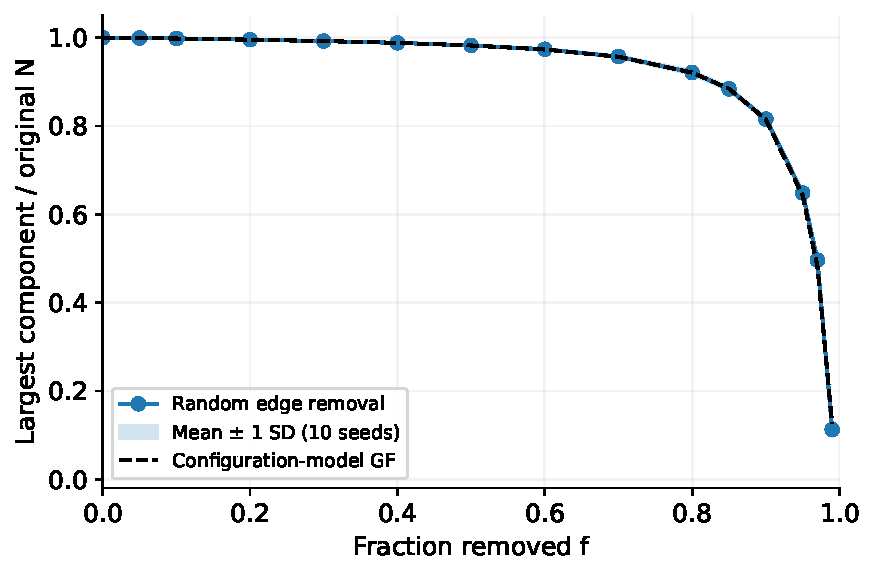
\includegraphics[width=\linewidth]{a_random_edge.pdf}
\caption{Edge removal.}
\end{subfigure}\hfill
\begin{subfigure}[t]{0.49\linewidth}
\centering
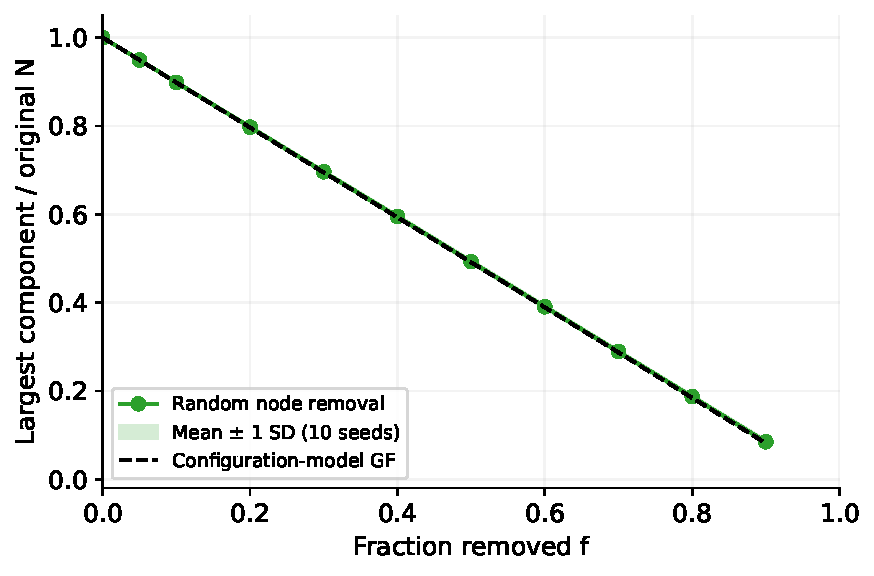
\includegraphics[width=\linewidth]{a_random_node.pdf}
\caption{Node removal.}
\end{subfigure}
\caption{Random-failure simulations on the 5,000-node graph; shading is the sample SD across ten seeds and dashed curves are configuration-model references.}
\label{fig:a-random}
\end{figure}

Under random node removal, S declines almost proportionally to the
surviving fraction over much of the range. At f=0.50, S$\approx$0.49252 means
about 98.5\% of surviving nodes belong to the largest component. A lower
node-removal curve than edge-removal curve does not by itself show
greater fragmentation at equal damage cost: deleted nodes directly
reduce the numerator and remove multiple incident edges. The fixed N0
denominator and additional surviving-edge counts make this distinction
explicit.

The GF reference tracks the main curves closely, with a more noticeable
bond difference at extreme removal. This is a quantitative observation
for this graph and these sample sizes, not proof that the network
satisfies configuration-model assumptions. We do not assign a unique
structural cause to the residual without further controls. The finite
graph and discrete damage grid also do not support an exact universal
critical threshold from curve shape alone.

\subsubsection{Sampling sensitivity and full-graph
comparison}\label{sampling-sensitivity-and-full-graph-comparison}

The filtered full graph gives a materially different bond curve. At
f=0.50, mean S$\approx$0.85830, compared with 0.98218 in the 5,000-node BFS
graph, a difference of approximately 0.124. At f=0.90, the corresponding
values are 0.55382 and 0.81540. These comparisons use the same damage
definition and ten seeds, but the graphs have different compositions and
permutation realizations; they are not paired measurements of identical
physical failures.

The full-graph result shows that the BFS subgraph overstates retention
of original nodes in the largest component for these damage levels.
Protein-rich sampling, degree changes and the removal of peripheral
parts of the full network are plausible contributors, but this
experiment alone does not isolate their separate effects. We therefore
present the 5,000-node curves as results for the agreed standard
subgraph and use the full graph to constrain claims about PrimeKG more
broadly. Figure~\ref{fig:a-sampling} displays this comparison.

\begin{figure}[htbp]
\centering
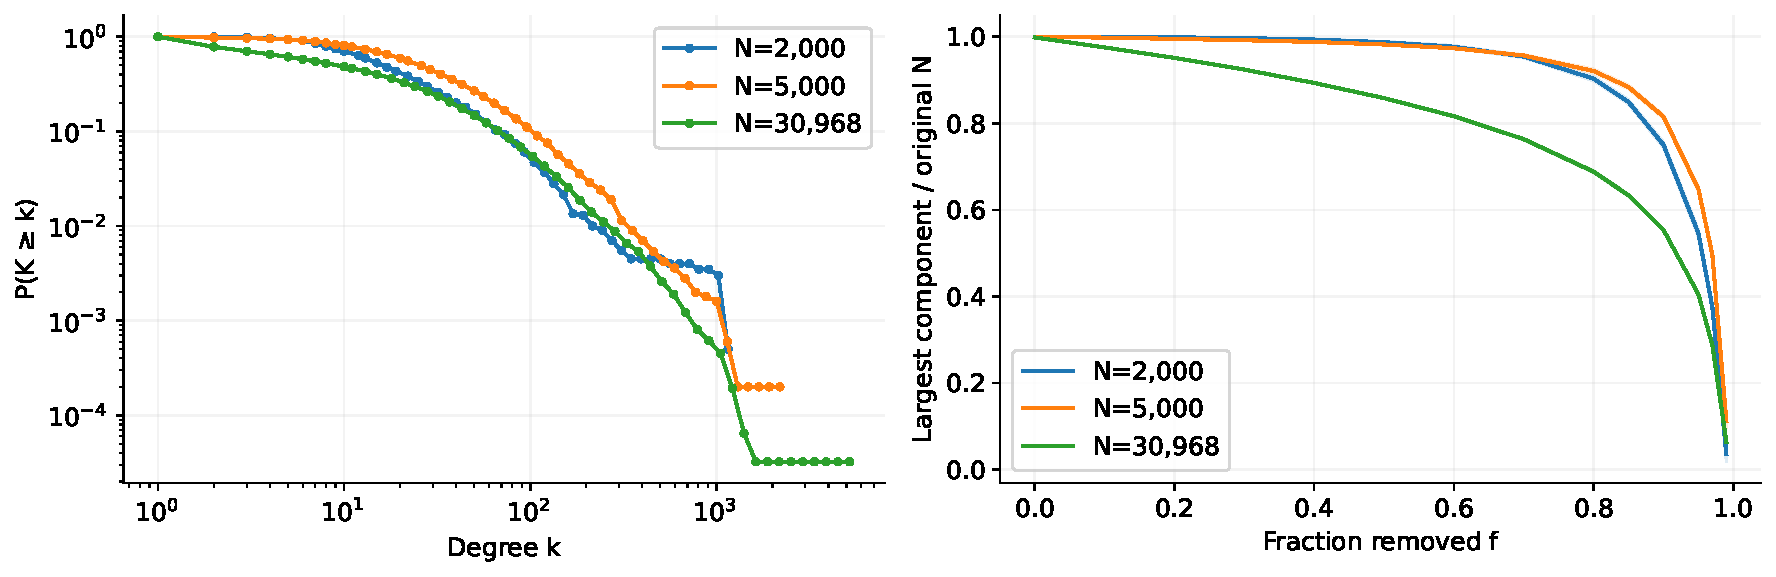
\includegraphics[width=0.82\linewidth]{a_sampling_comparison.pdf}
\caption{Random-edge robustness in the BFS samples and filtered full graph. The different graph constructions limit generalization from the 5,000-node sample.}
\label{fig:a-sampling}
\end{figure}

\subsubsection{Validation and connection to subsequent
workstreams}\label{validation-and-connection-to-subsequent-workstreams}

The union-find implementation was compared with independent NetworkX
calculations at every deletion state on 80 small random graphs,
including empty graphs and repeated semantic endpoint pairs. For each
real graph, independent checks at f=0, 0.3, 0.5, 0.9 and 1 cover both
edge and node deletion and six structural counts. The GF solver passes
the analytic 3-regular configuration-model identity. Separately, a clean
Python 3.11.9 rebuild reproduces all 68 core scientific
graph/query/order files byte-for-byte, including the shared BFS prefix.

For downstream retrieval and restoration, reference fixtures contain
endpoint survival, surviving two-hop path counts and PPI distances at
the same seed-0 damage states. They are computed independently with
NetworkX and can be used to validate C's retriever and E's zero-budget
baseline. The independent fixtures are distinct from the later C and E
integration checks documented elsewhere in the repository. This foundation allows the
subsequent sections to ask whether a structurally large component still
supports the fixed semantic tasks, and whether attacks or restoration
alter that relationship.
